\documentclass[conference]{IEEEtran}
\IEEEoverridecommandlockouts
\usepackage{cite}
\usepackage{float}
\usepackage{amsmath,amssymb,amsfonts}
\usepackage{graphicx}
\usepackage{textcomp}
\usepackage{xcolor}
\usepackage[utf8]{inputenc}
\usepackage[T1]{fontenc}
\usepackage{soul}
\usepackage[portuguese]{babel}
\usepackage{booktabs}
\usepackage{url}
\usepackage[export]{adjustbox}

\begin{document}

\title{Técnicas de Aprendizagem Automática para Previsão da Capacidade de Postos de Transformação}

\author{
\IEEEoverridecommandlockouts
\IEEEauthorblockN{Rui Santiago}
\IEEEauthorblockA{Dept. de Engenharia Informática \\
ISEP \\ Porto, Portugal \\ 1221402@isep.ipp.pt}
\and
\IEEEauthorblockN{Rui Silva}
\IEEEauthorblockA{Dept. de Engenharia Informática \\
ISEP \\ Porto, Portugal \\ 1231105@isep.ipp.pt}
\and
\IEEEauthorblockN{Tiago Barros}
\IEEEauthorblockA{Dept. de Engenharia Informática \\
ISEP \\ Porto, Portugal \\ 1231108@isep.ipp.pt}
}

\maketitle

% -------------------------------------------------------------------
\begin{abstract}
Este trabalho analisa, ao nível do PTD, o impacto da substituição de iluminação pública convencional por tecnologia LED na folga de potência disponível, avaliando a viabilidade técnica de realocar essa capacidade para infraestruturas de carregamento de veículos elétricos. Foram aplicadas técnicas de aprendizagem automática, nomeadamente regressão linear múltipla, árvores de decisão, SVM e redes neuronais, para a previsão contínua da folga de potência por PTD e para a classificação do nível de ocupação da rede. A avaliação foi conduzida com validação cruzada k-fold e os resultados comparados com testes de significância estatística. Para a regressão, a rede neuronal alcançou o melhor desempenho (MAE de 35,42 kVA). Para a classificação, a rede neuronal também se destacou com uma accuracy de 65,57\% e F1-score de 0,6490, superando os restantes modelos. Os resultados evidenciam que o perfil construtivo do PTD e a capacidade instalada são os preditores mais relevantes, e que as classes alta e baixa de ocupação representam o principal desafio de generalização para todos os modelos testados.
\end{abstract}

\begin{IEEEkeywords}
aprendizagem automática, postos de transformação, folga de potência, mobilidade elétrica, iluminação pública LED, redes neuronais, SVM, classificação, regressão
\end{IEEEkeywords}

% -------------------------------------------------------------------
\section{Introdução}

À medida que a emergência climática continua, a necessidade da descarbonização continua a exercer uma pressão crescente nas infraestruturas elétricas dos países europeus. A evolução rápida do mercado tecnológico apresenta ao mundo diversas tecnologias com um potential altamente disruptivo para as redes elétricas nacionais, e evidencia uma necessidade de preparar as mesmas para a chegada destas mudanças.

Dois setores nos quais estas mudanças disruptivas são bem ilustradas são a iluminação pública (IP) e os transportes pessoais. Em Portugal, a rede de IP representa uma porção significativa do consumo de eletricidade de municípios ao longo do país. No entanto, a adoção da tecnologia LED na rede de IP do país aumentou a eficiência da mesma no seu consumo de energia elétrica. E, simultaneamente, a crescente adoção do uso de veículos elétricos (VEs) pessoais tem aumentado a procura por estações de carregamento de VEs, necessitando a expansão da sua disponibilidade para impulsionar a adoção desta tecnologia a uma escala ainda maior.

Revela-se então uma clara oportunidade de sinergia, com a possibilidade de usar a potência libertada pela crescente otimização da rede de IP na expansão da rede de estações de carregamento de VEs.

\subsection{Objetivos}

O presente trabalho consiste numa análise e exploração de dados relativos á utilização dos cerca de 72\,000 Postos de Transformação de Distribuição (PTDs) da rede elétrica de baixa tensão portuguesa, fornecidos pela e-REDES~\cite{eredes}, com o objetivo de identificar em que locais do país existe uma oportunidade para a expansão da infraestrutura de estações de carregamento de VEs, com ou sem uma necessidade da modernização da sua rede de IP com tecnologias LED.

Para realizar esta exploração, pretende-se aplicar fundamentos de aprendizagem automática para desenvolver diversos modelos preditivos de regressão e classificação, com base em diversos algoritmos e mecanismos. Ao descobrir o modelo mais preciso, este poderá depois ser utilizado para simular como diferentes fatores, incluindo a porção da rede IP cujo usa iluminação LED eficiente, afetam a possibilidade da instalação de estações de carregamento de VEs, enquanto se evita a sobrecarga da rede elétrica.

Os objetivos específicos são: (i) realizar uma análise exploratória dos dados ao nível do PTD; (ii) desenvolver e comparar modelos de regressão para prever a folga de potência ($P_{Folga\_PTD}$); (iii) desenvolver e comparar modelos de classificação para o nível de ocupação da rede (utilizRede); (iv) selecionar, com suporte estatístico, o modelo com melhor desempenho em cada tarefa; e (v) realizar um estudo do impacto da modernização da rede de IP na viabilidade da expansão da rede de estações de carregamento de VEs.

\subsection{Uso de IA generativa}

Importa declarar que o desenvolvimento deste projeto contou com o auxílio de ferramentas de Inteligência Artificial generativa (nomeadamente os modelos Claude Sonnet 4.6 e Gemini 3.1). A sua utilização cingiu-se a um papel de assistente de redação, ajudando a reestruturar e a polir as nossas frases para garantir a adequação do tom e a clareza exigidas num artigo científico rigoroso. Adicionalmente, a IA tomou também um papel de apoio durante o desenvolvimento do código e desenvolvimento do dashboard interativo. Sublinhamos, contudo, que toda a formulação matemática, o pensamento analítico crítico, as tomadas de decisão na inferência estatística e as conclusões retiradas são da autoria exclusiva e integral do grupo.

% -------------------------------------------------------------------
\section{Estado da Arte}

\subsection{Aprendizagem Automática em Redes de Distribuição}

A aplicação de técnicas de aprendizagem automática (AA) a sistemas de energia elétrica tem crescido significativamente, impulsionada pela disponibilização de dados operacionais e pela maturação das ferramentas computacionais \cite{hippert2001}. Nos PTDs, ponto de convergência entre a rede de média tensão e os consumidores finais, a AA permite analisar a capacidade de absorção de novas cargas, como pontos de carregamento de VEs \cite{bishop2006}. Hippert et al.\ \cite{hippert2001} demonstraram que redes neuronais são competitivas com métodos estatísticos clássicos para previsão de carga, desde que treinadas com regularização adequada.

\subsection{Modelos de Regressão}

A \textbf{regressão linear múltipla} \cite{mitchell1997} estima coeficientes por mínimos quadrados ordinários (OLS), servindo como \textit{baseline} interpretável. A sua principal limitação é a assunção de linearidade entre preditores e resposta \cite{bishop2006}.

As \textbf{árvores de regressão} CART \cite{breiman1984} particionam recursivamente o espaço de \textit{features}, atribuindo a cada folha a média das respostas. A profundidade máxima controla a complexidade: árvores profundas favorecem \textit{overfitting}, rasas incorrem em \textit{underfitting}. A sua interpretabilidade permite identificar variáveis discriminativas.

O \textbf{SVR} \cite{vapnik1995} estende a maximização de margem do SVM à regressão, aprendendo uma função que aproxima os alvos dentro de um tubo de insensibilidade $\varepsilon$. O parâmetro $C$ equilibra regularização e penalização de erros. A variante linear é eficiente computacionalmente; o kernel RBF permite modelar não-linearidades a maior custo \cite{cortes1995}.

As \textbf{redes neuronais} MLP (\textit{Multilayer Perceptron}) \cite{haykin1999} são aproximadores universais de funções. O treino por retropropagação \cite{rumelhart1986} minimiza o erro quadrático médio. A regularização L2 e o \textit{early stopping} são mecanismos essenciais para mitigar o \textit{overfitting} \cite{goodfellow2016}.

\subsection{Modelos de Classificação}

As \textbf{árvores de classificação} CART \cite{breiman1984} selecionam divisões que maximizam a redução de impureza (índice de Gini ou entropia \cite{quinlan1986}), servindo simultaneamente como ferramenta de análise de importância de variáveis.

O \textbf{SVM de classificação} \cite{cortes1995} determina o hiperplano de margem máxima entre classes. Para problemas multiclasse, a estratégia \textit{One-vs-Rest} treina $K$ classificadores binários independentes. O LinearSVC é escalável a \textit{datasets} de grande dimensão \cite{pedregosa2011}.

Para classificação multiclasse, o \textbf{MLP} utiliza a função \textit{softmax} na camada de saída para produzir probabilidades de classe, com a entropia cruzada como função de perda. Ativações ReLU permitem capturar fronteiras de decisão não-lineares \cite{goodfellow2016}.

O \textbf{KNN} \cite{cover1967} classifica cada observação pela classe mais frequente entre os $k$ vizinhos mais próximos. O parâmetro $k$ controla o equilíbrio \textit{bias-variance} e a normalização das \textit{features} é imprescindível.

\subsection{Avaliação e Validação}

A \textbf{validação cruzada} $k$-\textit{fold} \cite{kohavi1995} produz estimativas de desempenho estáveis, treinando e avaliando o modelo em $k$ partições distintas. Para regressão, utilizam-se MAE e RMSE; para classificação, \textit{Accuracy}, \textit{Precision}, \textit{Recall} e F1-\textit{score} \cite{bishop2006}. A significância das diferenças entre modelos é verificada por t-\textit{test} pareado ou, na ausência de normalidade (teste de Shapiro-Wilk), pelo teste de Wilcoxon \cite{mitchell1997}.

% -------------------------------------------------------------------
\section{Metodologia}

\subsection{Dataset e Variáveis}

O dataset disponibilizado pela e-REDES, PTD\_level\_dataset.xlsx, resulta da junção de dados de iluminação pública e de postos de transformação, pelo concelho onde se localiza o PTD. Contém aproximadamente 72\,000 registos com as variáveis descritas na Tabela~\ref{tab:variaveis}.

\begin{table}[H]
\caption{Variáveis do Dataset}
\label{tab:variaveis}
\begin{center}
\begin{tabular}{lll}
\toprule
Nível PTD & Agregadas Concelho & Derivadas \\
\midrule
Cap\_PTD\_kVA & P\_IP\_Total & PFolga\_PTD \\
N\_Clientes & Rate\_Ineficiencia & Cap\_per\_Cliente \\
Pot\_Contratada\_kVA & LED\_Ratio & IP\_per\_PTD \\
Tipo\_Construtivo & & \\
\bottomrule
\end{tabular}
\end{center}
\end{table}

As variáveis derivadas calculadas incluem também as variáveis-alvo do projeto: O Ganho LED ($\Delta P_{LED}$), uma medida da potência libertada pelo uso de tecnologias LED, a Folga da Rede ($P_{Folga}$), a potência usada na Carga de VEs ($P_{VE}$) e o Saldo Final de Viabilidade ($D$), em relação á instalação de estações de carregamento de VEs. Uma outra variável-alvo, utilizRede, foi obtida por discretização da percentagem de uso de PTDs, medida com uma variável adicional presente, Util\_Decimal, em três classes (baixo, médio, alto) com base em limiares fixos ($\leq 0{,}33$, $0{,}33$--$0{,}66$, $> 0{,}66$),.

\subsection{Pré-processamento}

O pré-processamento incluiu: (i) remoção de registos com valores omissos nas variáveis-alvo; (ii) transformação de variáveis categóricas (por exemplo, o distrito e concelho) em variáveis numéricas; (iii) normalização dos dados para SVM e redes neuronais; (iv) seleção de variáveis relevantes para o treino dos modelos preditivos, e remoção de todas as variáveis irrelevantes.

Esta seleção resultou na seguinte lista de 10 variáveis, que exclui as variáveis-alvo descritas anteriormente: A potência instalada em um PTD (Potência Instalada [kVA]), o número de clientes (N\_Clientes), a potência total usada em IP (P\_IP\_Total), a potência usada em IP ineficiente (P\_IP\_Inef), o rácio de uso de tecnologias LED na IP correspondente (LED\_Ratio), o número de luminárias correspondente (N\_Luminarias), o número de lâmpadas correspondente (N\_Lampadas), a capacidade necessária por cliente (Cap\_per\_Cliente), o distrito correspondente (Distrito\_enc), e o concelho correspondente (Concelho\_enc). Os modelos explorados serão treinados para utilizar este conjunto de variáveis, ou parte dele, para determinar as variáveis-alvo.

% -------------------------------------------------------------------
\section{Análise Exploratória de Dados}

A Fig.~\ref{fig:distribuicao} apresenta a distribuição das principais variáveis. A variável LED\_Ratio exibe uma assimetria que sugere que a maior parte da rede de IP do país já se encontra com níveis elevados de utilização de tecnologia LED, no entanto, ainda existe um número considerável de ocorrências de valores inferiores. A variável Util\_Decimal concentra-se entre 0,2 e 0,6, sinalizando uma rede elétrica nacional em média subcarregada e com uma grande capacidade extra para a expansão da oferta de estações de carregamento de VEs.

\begin{figure}[H]
\centerline{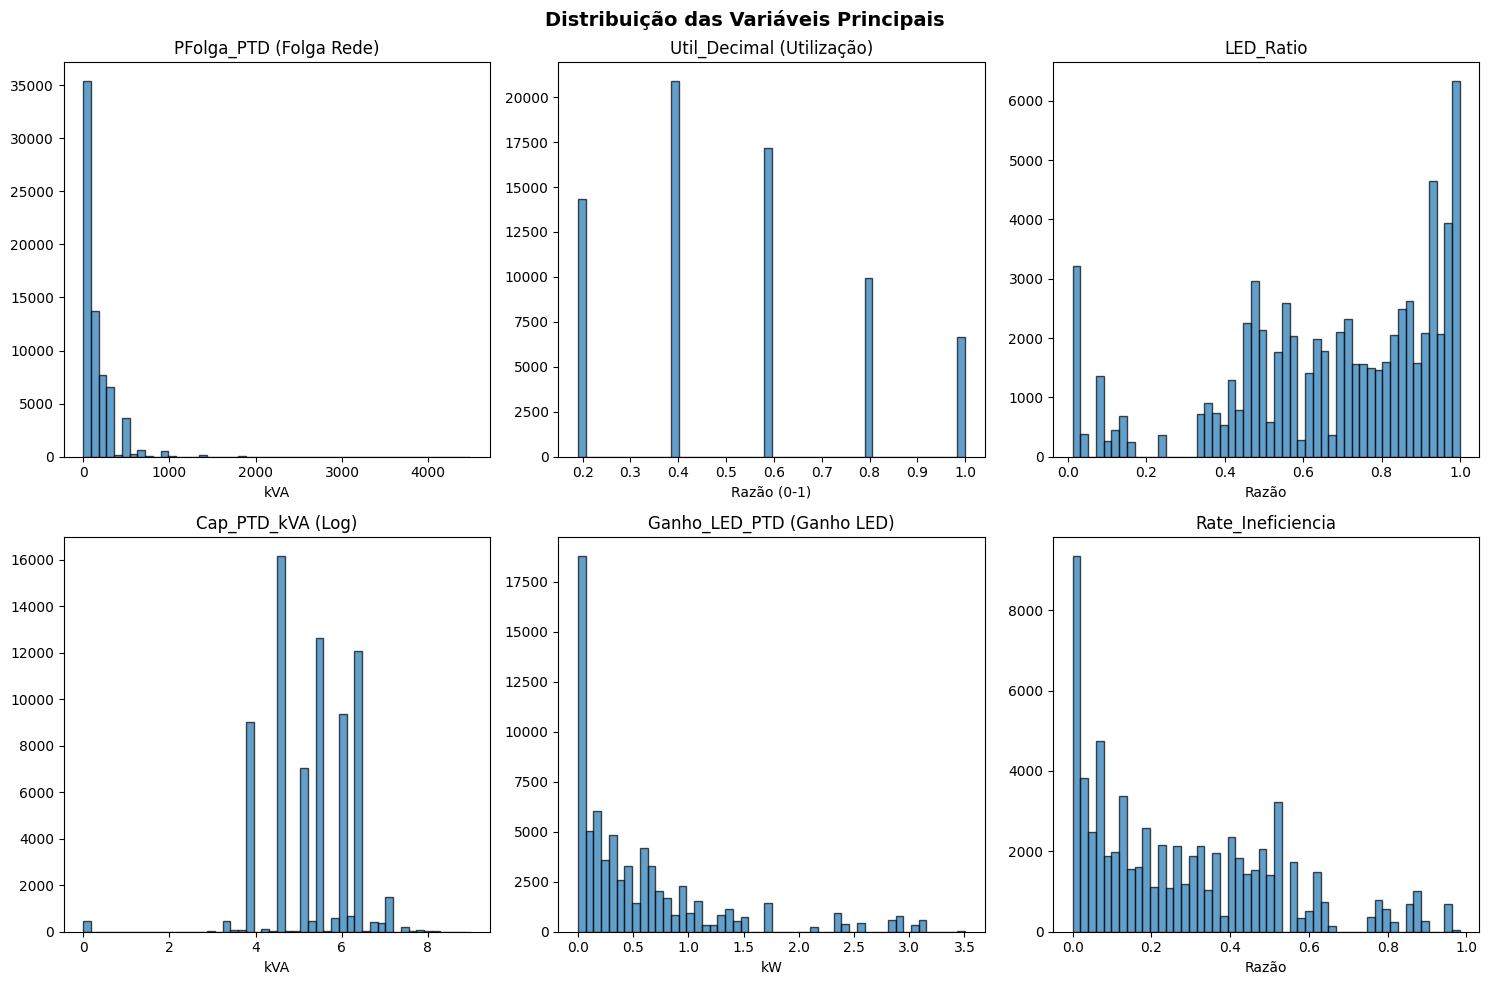
\includegraphics[width=\columnwidth]{./img/distribuicao_variaveis.png}}
\caption{Distribuição das principais variáveis do dataset.}
\label{fig:distribuicao}
\end{figure}

A análise por distrito (Fig.~\ref{fig:distrito}) revela uma heterogeneidade geográfica considerável, com distritos do interior a apresentar um nível de utilização inferior à tendência do resto do país. No entanto, nenhum distrito apresenta uma rede elétrica perto de saturação máxima.

\begin{figure}[H]
\centerline{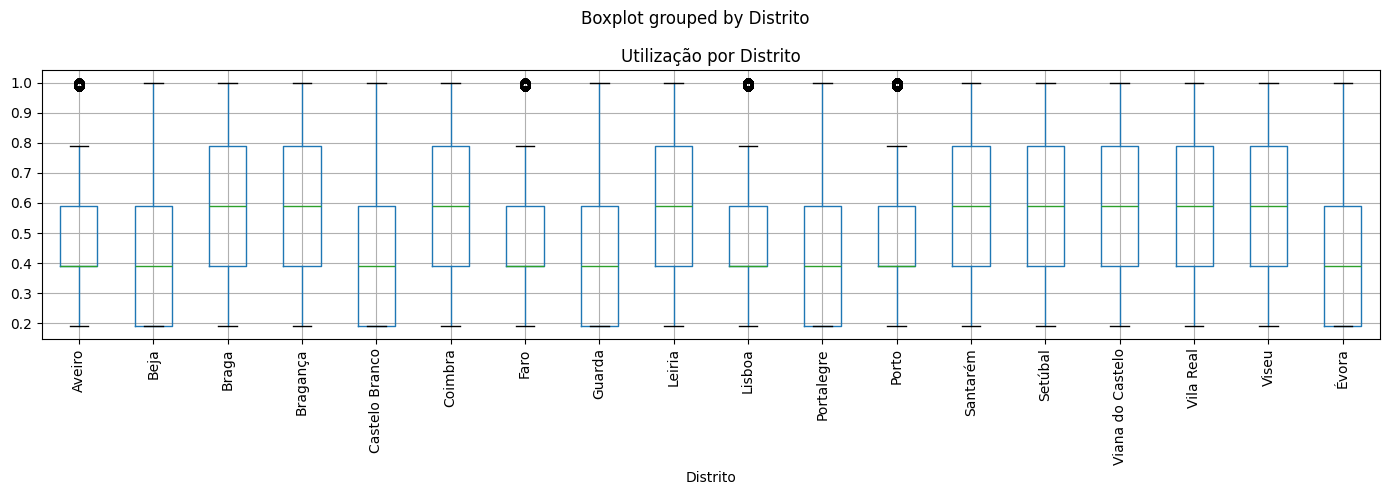
\includegraphics[width=\columnwidth]{./img/utilizacao_distrito.png}}
\caption{Utilização da rede por distrito.}
\label{fig:distrito}
\end{figure}

A correlação entre variáveis (Fig.~\ref{fig:corr_dataset}) confirma que a Potência Instalada [kVA] e a capacidade por cliente são os preditores mais correlacionados com $P_{Folga\_PTD}$, enquanto variáveis de iluminação pública (N\_Lampadas, N\_Luminárias) apresentam correlação moderada. Isto sugere que a rede de IP pode não estar entre os fatores mais consequentes na folga da rede elétrica, embora o seu contributo não seja negligenciável.

\begin{figure}[H]
\centerline{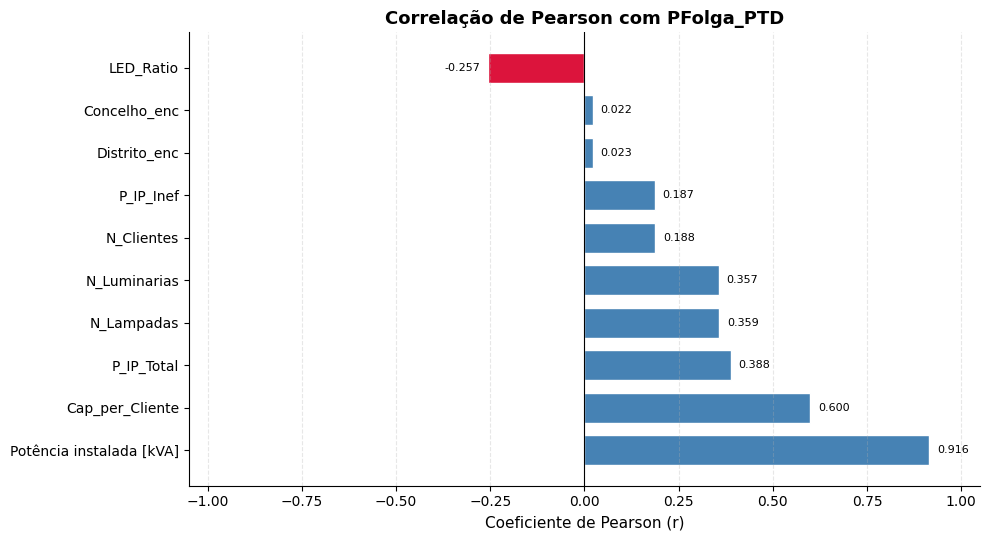
\includegraphics[width=\columnwidth]{./img/correlacao_de_pearson_folga.png}}
\caption{Matriz de correlação do dataset.}
\label{fig:corr_dataset}
\end{figure}

% -------------------------------------------------------------------
\section{Regressão: Previsão de $P_{Folga\_PTD}$}

\subsection{Regressão Linear Simples}

Como variável explicativa para a regressão linear simples foi selecionada a Potência Instalada [kVA], por apresentar a correlação de Pearson mais elevada com $P_{Folga\_PTD}$ (Fig.~\ref{fig:corr_dataset}). Esta escolha é objetivamente justificável: a folga de potência de um PTD é, por definição, a diferença entre a capacidade instalada e a carga efetivamente utilizada, pelo que a capacidade instalada é o preditor individual com maior poder explicativo linear. A Fig.~\ref{fig:reg_linear} ilustra a reta ajustada e o diagrama de dispersão correspondente. A dispersão residual considerável evidencia que um único preditor linear é insuficiente para capturar a complexidade do fenómeno, motivando o desenvolvimento de modelos múltiplos.

\begin{figure}[H]
\centerline{
\includegraphics[width=\columnwidth]{./img/pesado/regressao_linear_simples.png}}
\caption{Regressão linear simples: $P_{Folga\_PTD}$ em função da Potência Instalada [kVA].}
\label{fig:reg_linear}
\end{figure}

\subsection{Motivação e Seleção dos Modelos de Regressão Múltipla}

A escolha dos quatro modelos decorre de critérios complementares, considerando as características do problema: elevada dimensionalidade, presença de variáveis categóricas codificadas, e relações presumivelmente não-lineares entre a folga de potência e os preditores. A regressão linear múltipla serve como baseline interpretável. Ao assumir uma relação linear e aditiva com a variável $P_{Folga\_PTD}$, este modelo estabelece uma base de comparação para quantificar o ganho de desempenho dos algoritmos mais complexos, além de fornecer coeficientes diretamente interpretáveis em termos operacionais. A sua limitação fundamental é a incapacidade de capturar interações e não-linearidades, que é precisamente o que os modelos seguintes visam superar. 

A árvore de regressão foi selecionada pela sua capacidade de segmentar o espaço de features em grupos com comportamentos distintos, como PTDs industriais e residenciais, mantendo simultaneamente uma estrutura interpretável. Foi utilizada uma profundidade máxima de 10 níveis para capturar a heterogeneidade dos dados e limitar o overfitting.

O SVM de regressão (LinearSVR) foi escolhido pela sua capacidade de generalização em dados ruidosos, através da regularização e da tolerância a erros definida por $\varepsilon$. A variante linear foi adotada por razões de escalabilidade, sendo testados três valores de $C$ ($0{,}1$, $1{,}0$ e $10{,}0$) para avaliar diferentes níveis de regularização.

A rede neuronal (MLPRegressor) foi utilizada pela sua capacidade de modelar relações não lineares e interações complexas entre variáveis. Foram avaliadas três configurações com complexidade crescente (Tabela~\ref{tab:nn_configs_reg}), variando o número de camadas, neurónios e regularização L2, mantendo constantes a learning rate ($\eta = 0{,}001$) e o mecanismo de early stopping ($n\_iter\_no\_change = 10$).

\begin{table}[H]
\caption{Configurações da Rede Neuronal na Regressão}
\label{tab:nn_configs_reg}
\begin{center}
\begin{tabular}{lccc}
\toprule
Configuração & Arquitetura & $\alpha$ (L2) \\
\midrule
Rasa       & (64)        & $10^{-4}$ \\
Média      & (128, 64)   & $10^{-3}$ \\
Profunda   & (256, 128, 64) & $10^{-2}$ \\
\bottomrule
\end{tabular}
\end{center}
\end{table}

As curvas de loss de treino e validação para as três configurações são apresentadas na Fig.~\ref{fig:curvas_loss_reg}. A configuração rasa converge rapidamente mas estabiliza com loss superior, sugestivo de underfitting: a capacidade expressiva de uma única camada de 64 neurónios é insuficiente para modelar as interações entre as variáveis de consumo e capacidade. A configuração profunda apresenta um gap ligeiro entre treino e validação nos primeiros epochs, atenuado progressivamente pela regularização L2 elevada ($\alpha = 0{,}01$) e pelo early stopping, que interrompeu o treino ao detetar estagnação da loss de validação. A configuração profunda (três camadas, L2 forte) atingiu o melhor equilíbrio bias-variance, com convergência das curvas e loss de validação mínima. O early stopping revelou-se crítico: sem ele, a configuração profunda exibiria overfitting crescente após os primeiros epochs de estabilização.

\begin{figure}[H]
\centerline{
\includegraphics[width=\columnwidth]{./img/pesado/curvas_loss_nn.png}}
\caption{Curvas de loss treino e validação das três configurações da rede neuronal para regressão.}
\label{fig:curvas_loss_reg}
\end{figure}

\subsection{Resultados e Comparação dos Modelos de Regressão}

A Tabela~\ref{tab:regressao} resume os resultados de todos os modelos com k-fold ($k=10$).

\begin{table}[H]
\caption{Resultados de Regressão (Perfil Pesado, k-fold $k=10$)}
\label{tab:regressao}
\begin{center}
\begin{tabular}{lcccc}
\toprule
Modelo & MAE & $\pm$ & RMSE & $\pm$ \\
\midrule
Linear     & 37,50 & 0,47 & 57,31 & 1,25 \\
Tree       & 36,28 & 0,35 & 58,72 & 1,72 \\
SVM        & 36,72 & 0,41 & 59,38 & 1,35 \\
NeuralNet  & 35,42 & 0,45 & 55,35 & 1,63 \\
\bottomrule
\end{tabular}
\end{center}
\end{table}

A rede neuronal obteve o menor MAE (35,42 kVA) e RMSE (55,35 kVA), confirmando a sua superior capacidade de aproximação das relações não-lineares entre os preditores e a folga de potência.

O modelo linear apresentou o pior MAE (37,50 kVA), evidenciando que a relação entre os preditores e $P_{Folga\_PTD}$ não é puramente linear, a capacidade instalada e o número de clientes interagem de forma não-linear com as características geográficas e de consumo dos PTDs. A árvore de regressão melhorou o MAE face ao modelo linear (36,28 kVA) ao capturar partições do espaço de features, mas exibiu RMSE superior (58,72 kVA), indicando maior sensibilidade a erros pontuais elevados, um comportamento esperado em árvores sem boosting, que produzem previsões constantes por folha e podem falhar em PTDs com perfis atípicos. O SVM posicionou-se entre a árvore e o modelo linear em MAE (36,72 kVA), mas apresentou o pior RMSE (59,38 kVA). Este resultado sugere que a linearidade do kernel, embora eficiente computacionalmente, não captura adequadamente as não-linearidades mais complexas do problema; um kernel RBF poderia melhorar o desempenho à custa de maior custo computacional. A rede neuronal destacou-se em ambas as métricas, com os menores MAE e RMSE. A sua arquitetura de três camadas ocultas (256, 128 e 64 neurónios) com regularização L2 forte demonstrou ser suficientemente expressiva para modelar as interações entre variáveis de consumo, capacidade e iluminação pública, sem incorrer em overfitting.

\subsection{Curvas de Aprendizagem}

As curvas de aprendizagem dos dois melhores modelos de regressão (NeuralNet e Tree) são apresentadas na Fig.~\ref{fig:curvas_reg}. A rede neuronal apresenta uma diferença reduzida entre os erros de treino e validação ao longo de todo o processo de aprendizagem. Para o maior conjunto de treino, o MAE estabiliza em aproximadamente 34,9~kVA no treino e 35,3~kVA na validação, correspondendo a um gap inferior a 0,5~kVA. Este comportamento sugere boa capacidade de generalização e ausência de sinais relevantes de overfitting. Além disso, observa-se uma estabilização gradual das curvas à medida que aumenta o número de amostras, indicando que o modelo já beneficia menos de dados adicionais.

A árvore de decisão apresenta um comportamento distinto. Embora o erro de validação diminua de forma consistente com o aumento dos dados de treino, mantém-se uma diferença significativa relativamente ao erro de treino, superior a 4~kVA para os maiores conjuntos de dados. Este padrão sugere uma capacidade de generalização inferior à da rede neuronal e evidencia uma variância mais elevada do modelo. Ainda assim, a redução progressiva do erro de validação indica que a disponibilidade de mais dados contribui para melhorar o seu desempenho.

\begin{figure}[H]
\centerline{
\includegraphics[width=\columnwidth]{./img/pesado/curvas_aprendizagem_regressao.png}}
\caption{Curvas de aprendizagem para NeuralNet e Tree em regressão.}
\label{fig:curvas_reg}
\end{figure}

\subsection{Teste de Significância Estatística}

Aplicou-se o t-test pareado entre NeuralNet e Decision Tree, após confirmação de normalidade das distribuições de erro por fold pelo teste de Shapiro-Wilk. O resultado ($t = 3{,}04$; $p = 0{,}0141 < 0{,}05$) confirma que a diferença é estatisticamente significativa ($\alpha = 0.05$). O modelo NeuralNet é o melhor modelo de regressão.

% -------------------------------------------------------------------
\section{Classificação: Previsão de utilizRede}

\subsection{Definição das Classes}

A variável utilizRede foi derivada de Util\_Decimal por discretização com limiares fixos ($Q_{33\%} = 0{,}33$ e $Q_{67\%} = 0{,}66$), originando três classes: baixo ($\leq 0{,}33$), médio ($0{,}33$--$0{,}66$) e alto ($> 0{,}66$). Esta abordagem garante interpretabilidade operacional direta, cada classe corresponde a um regime de utilização da rede com implicações distintas para a instalação de pontos de carregamento, e produz uma distribuição suficientemente equilibrada entre classes para suportar classificadores multiclasse sem recurso a técnicas de oversampling.

\subsection{Motivação e Seleção dos Modelos de Classificação}

A tarefa de classificação de utilizRede apresenta características distintas da regressão: as fronteiras de decisão entre classes adjacentes (especialmente médio-baixo e médio-alto) são difusas por construção, exigindo modelos com capacidade de capturar zonas de transição graduais. A árvore de decisão é justificada pelo seu duplo papel: classificador e ferramenta de análise de importância de features. A estrutura hierárquica de divisões permite identificar quais os atributos que mais discriminam os três regimes de utilização, complementando a análise de correlação linear. Com $\mathrm{max\_depth} = 10$, o modelo captura fronteiras de decisão não-lineares sem memorizar exemplos individuais.

O SVM (LinearSVC) foi selecionado pela sua capacidade de encontrar fronteiras de decisão lineares em espaços de features de elevada dimensão, beneficiando simultaneamente de mecanismos de regularização que promovem a generalização. O parâmetro de regularização $C$ foi testado para os valores $0{,}1$, $1{,}0$ e $10{,}0$, permitindo avaliar diferentes compromissos entre margem e erros de classificação. A variante linear foi preferida pela sua eficiência computacional e escalabilidade para conjuntos de dados de grande dimensão.

O KNN foi incluído como método de referência não paramétrico. O modelo classifica cada PTD com base nos seus $k$ vizinhos mais próximos no espaço de features normalizadas, capturando padrões locais sem assumir uma forma funcional específica para a fronteira de decisão. O parâmetro $k$ foi otimizado por grid search em $\{3,5,7,11,15\}$, sendo a normalização das features essencial devido à utilização da distância euclidiana.

Tal como na regressão, as três configurações da rede neuronal (Tabela~\ref{tab:nn_configs_clf}) foram avaliadas com curvas de loss de treino e validação (Fig.~\ref{fig:curvas_loss_clf}).

\begin{table}[H]
\caption{Configurações da Rede Neuronal na Classificação}
\label{tab:nn_configs_clf}
\begin{center}
\begin{tabular}{lccc}
\toprule
Configuração & Arquitetura & $\alpha$ (L2) \\
\midrule
Rasa       & (64)        & $10^{-4}$ \\
Média      & (128, 64)   & $10^{-3}$ \\
Profunda   & (256, 128, 64) & $10^{-2}$ \\
\bottomrule
\end{tabular}
\end{center}
\end{table}

\begin{figure}[H]
\centerline{
\includegraphics[width=\columnwidth]{./img/pesado/curvas_loss_nn_classificacao.png}}
\caption{Curvas de loss treino e validação das três configurações da rede neuronal para classificação.}
\label{fig:curvas_loss_clf}
\end{figure}

As curvas de loss revelam um padrão consistente com a regressão: a configuração rasa atinge um patamar elevado rapidamente (underfitting), enquanto a configuração profunda apresenta um gap inicial entre treino e validação que o early stopping mitiga. A configuração profunda (3 camadas, L2 forte) apresenta curvas convergentes, sendo selecionada como melhor configuração.

\subsection{Resultados Globais e Comparação de Modelos}

A Tabela~\ref{tab:classificacao} resume as métricas globais com k-fold ($k=10$). A rede neuronal superou todos os modelos em todas as métricas globais, enquanto o SVM revelou o pior desempenho.

\begin{table}[H]
\caption{Resultados de Classificação (Perfil Pesado, k-fold $k=10$)}
\label{tab:classificacao}
\begin{center}
\begin{tabular}{lcccc}
\toprule
Modelo & Acc & $\pm$ & F1 & $\pm$ \\
\midrule
Decision Tree & 0,6477 & 0,0059 & 0,6418 & 0,0059 \\
NeuralNet     & 0,6557 & 0,0082 & 0,6490 & 0,0092 \\
SVM           & 0,5934 & 0,0072 & 0,5168 & 0,0097 \\
KNN           & 0,6393 & 0,0077 & 0,6344 & 0,0075 \\
\bottomrule
\end{tabular}
\end{center}
\end{table}

Em termos de accuracy, a rede neuronal atingiu 65,57\%, correspondendo a 0,80 pontos percentuais acima da árvore de decisão (64,77\%), 1,64 pp acima do KNN (63,93\%) e 6,23 pp acima do SVM (59,34\%). Em F1-score, a rede neuronal (0,6490) apresenta a melhor média harmónica entre precision e recall, seguida da árvore de decisão (0,6418) e do KNN (0,6344). O SVM destaca-se negativamente com F1 de apenas 0,5168, penalizado em particular nas classes extremas onde apresenta recall muito reduzido, um claro sintoma de underfitting: o modelo linear não tem capacidade suficiente para delinear as fronteiras de decisão, classificando a maioria das instâncias na classe médio (recall$_{\mathrm{médio}} = 0{,}94$, recall$_{\mathrm{alto}} = 0{,}19$, recall$_{\mathrm{baixo}} = 0{,}14$).

\subsection{Desempenho por Classe}

A Fig.~\ref{fig:f1_classe} apresenta o F1-score por classe para cada modelo. Observa-se que a classe \textit{médio} é consistentemente a mais fácil de classificar, atingindo valores de F1 próximos de 0,72 para a NeuralNet, Decision Tree e SVM. Em contraste, as classes \textit{alto} e \textit{baixo} apresentam desempenhos substancialmente inferiores, com F1 entre 0,50 e 0,61 nos melhores modelos.

Este comportamento sugere que a classe \textit{médio} possui padrões mais consistentes e/ou maior representação no conjunto de dados, facilitando a aprendizagem das fronteiras de decisão. Pelo contrário, as classes extremas apresentam maior dificuldade de separação, possivelmente devido à menor representatividade e à sobreposição das suas características com as da classe intermédia.

A NeuralNet obtém o melhor desempenho global, alcançando o maior F1 nas classes \textit{alto} (0,606) e \textit{médio} (0,722). A Decision Tree apresenta o melhor resultado na classe \textit{baixo} (0,513), embora a diferença para a NeuralNet seja reduzida. O SVM evidencia um forte desequilíbrio de desempenho entre classes, obtendo resultados competitivos para a classe \textit{médio} (0,719), mas degradando significativamente nas classes \textit{alto} (0,300) e \textit{baixo} (0,229), o que sugere uma maior dificuldade em identificar as classes minoritárias.

\begin{figure}[H]
\centerline{
\includegraphics[width=\columnwidth]{./img/pesado/f1score_por_classe_modelo.png}}
\caption{F1-score por classe e por modelo em classificação.}
\label{fig:f1_classe}
\end{figure}

A Fig.~\ref{fig:conf_matrix} apresenta a matriz de confusão do melhor modelo, uma Rede Neural Profunda com três camadas ocultas e regularização L2 forte. A classe \textit{médio} é a mais bem identificada, com \textit{recall} de 78\%, enquanto as classes \textit{alto} e \textit{baixo} apresentam \textit{recalls} de 53\% e 47\%, respetivamente.

Os principais erros ocorrem na classificação das classes \textit{alto} e \textit{baixo} como \textit{médio}, sugerindo que esta última funciona como uma categoria intermédia no espaço de características. Em particular, 42\% das amostras \textit{alto} e 51\% das amostras \textit{baixo} são classificadas como \textit{médio}. Em contraste, a confusão direta entre \textit{alto} e \textit{baixo} é reduzida.

\begin{figure}[H]
\centerline{
\includegraphics[width=\columnwidth]{./img/pesado/matriz_de_confusao.png}}
\caption{Matriz de confusão da rede neuronal para classificação.}
\label{fig:conf_matrix}
\end{figure}

\subsection{Importância de Variáveis e Comparação com Correlações}

A Fig.~\ref{fig:feat_imp} compara a importância das variáveis obtida através da árvore de decisão com a correlação linear de Pearson relativamente a \textit{utilizRede}. Esta análise permite identificar variáveis relevantes tanto em relações lineares como não lineares com a variável alvo.

\begin{figure}[H]
\centerline{
\includegraphics[width=\columnwidth]{./img/pesado/importancia_feature_vs_correlacao_utilzRede.png}}
\caption{Importância de variáveis da árvore de decisão vs correlação de Pearson com \textit{utilizRede}.}
\label{fig:feat_imp}
\end{figure}

As variáveis \textit{Cap\_per\_Cliente} e \textit{N\_Clientes} destacam-se em ambos os métodos, evidenciando elevado poder preditivo e uma relação consistente com o nível de utilização da rede. Por sua vez, a \textit{Potência instalada [kVA]} apresenta a maior correlação linear, mas uma importância relativamente inferior na árvore, sugerindo que parte do seu efeito é capturado através de interações com outras variáveis.

Em contraste, variáveis geográficas, como \textit{Distrito\_enc} e \textit{Concelho\_enc}, exibem baixa correlação linear, mas mantêm importância não negligenciável no modelo baseado em árvore. Este comportamento indica a existência de relações não lineares e efeitos de interação que não são capturados pela correlação de Pearson. Assim, a comparação entre ambos os métodos fornece uma visão complementar da relevância das variáveis e evidencia a utilidade de abordagens não lineares na modelação da ocupação da rede.

\subsection{Curvas de Aprendizagem}

A Fig.~\ref{fig:curvas_class} apresenta as curvas de aprendizagem do melhor modelo (NeuralNet) e do pior modelo (SVM). A NeuralNet exibe curvas de treino e validação próximas e estáveis, convergindo para valores de F1 de aproximadamente 0,66 e 0,65, respetivamente. O reduzido desfasamento entre ambas sugere boa capacidade de generalização e ausência de sobreajuste significativo.

Em contraste, o SVM apresenta curvas praticamente sobrepostas, mas estabilizadas em valores de F1 mais baixos (cerca de 0,52). Este comportamento é indicativo de \textit{underfitting}, sugerindo que o modelo possui capacidade limitada para capturar os padrões presentes nos dados. Além disso, o desempenho permanece praticamente inalterado com o aumento do número de amostras, indicando que a inclusão de mais dados dificilmente resultaria em melhorias substanciais.

\begin{figure}[H]
\centerline{
\includegraphics[width=\columnwidth]{./img/pesado/curvas_aprendizagem_class.png}}
\caption{Curvas de aprendizagem para NeuralNet e SVM em classificação.}
\label{fig:curvas_class}
\end{figure}

\subsection{Teste de Significância Estatística}

O t-test pareado entre NeuralNet e Decision Tree ($t = 3{,}04$; $p = 0{,}0141 < 0{,}05$) confirma diferença estatisticamente significativa no F1-score ($\alpha = 0.05$). O modelo NeuralNet é o melhor modelo de classificação.

% -------------------------------------------------------------------
\section{Discussão}

\subsection{Comparação de Perfis e Trade-off Desempenho–Tempo}

Os resultados apresentados até aqui (Figuras e Tabelas) referem-se exclusivamente ao perfil pesado, que incorpora o conjunto mais completo de variáveis e a maior dimensão amostral. Para contextualizar o trade-off associado, os modelos foram também treinados nos perfis leve e médio. A Tabela~\ref{tab:perfis_reg} e a Figura~\ref{fig:comparacao_accuracy_f1} \,sintetizam os resultados da regressão.

\begin{table}[H]
\caption{MAE (kVA) por perfil e modelo.}
\label{tab:perfis_reg}
\centering
\begin{tabular}{lccc}
\toprule
Modelo & Leve & Médio & Pesado \\
\midrule
Regressão Linear & 37,52 & 37,50 & 37,50 \\
Árvore Decisão   & 36,37 & 36,38 & 36,28 \\
SVM              & 36,73 & 36,72 & 36,72 \\
Rede Neuronal    & 36,03 & 35,66 & \textbf{35,42} \\
\bottomrule
\end{tabular}
\end{table}

Observa-se uma melhoria consistente com o aumento do detalhe dos dados, especialmente para a rede neuronal (redução de MAE de 36,03 para $35{,}42$kVA). Em classificação (Tabela~\ref{tab:perfis_clf}), a rede neuronal também apresenta o melhor resultado no perfil pesado (F1 de 0,6490), superando os restantes modelos. A Figura~\ref{fig:comparacao_accuracy_f1} ilustra estas diferenças.

\begin{table}[H]
\caption{F1-score por perfil e modelo.}
\label{tab:perfis_clf}
\centering
\begin{tabular}{lccc}
\toprule
Modelo & Leve & Médio & Pesado \\
\midrule
Árvore Decisão & 0,6038 & 0,6313 & 0,6418 \\
Rede Neuronal & 0,6169 & 0,6482 & \textbf{0,6490} \\
SVM           & 0,5305 & 0,5422 & 0,5168 \\
KNN           & 0,5679 & 0,6132 & 0,6344 \\
\bottomrule
\end{tabular}
\end{table}

\begin{figure}[H]
\centering
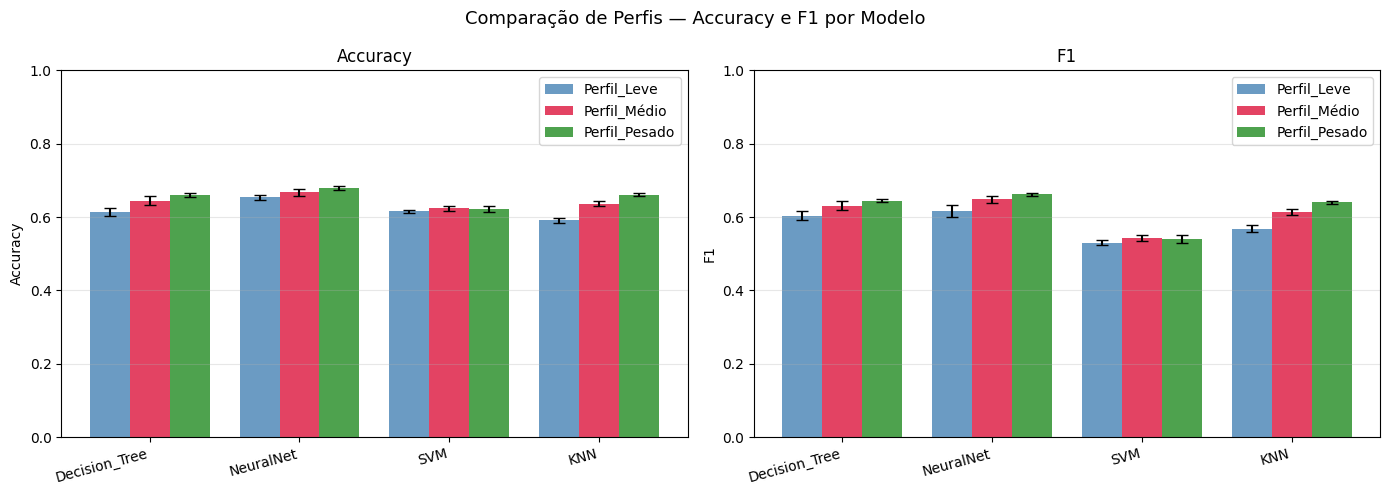
\includegraphics[width=\columnwidth]{img/comparisons/comparacao_accuracy_f1.png}
\caption{Accuracy (esquerda) e F1-score (direita) por modelo no perfil pesado.}
\label{fig:comparacao_accuracy_f1}
\end{figure}

A melhoria de desempenho do perfil pesado tem um custo computacional elevado: o treino da rede neuronal no perfil pesado demora cerca de 4 horas, contra apenas 10 minutos no perfil leve. Para aplicações sensíveis à latência ou com recursos limitados, o perfil médio com árvore de decisão oferece um compromisso razoável (MAE de $36{,}38$kVA, apenas $0{,}96$kVA acima do melhor modelo, com tempo de treino muito inferior).

\subsection{Análise Global e Limitações}

Os resultados mostram que a rede neuronal é consistentemente superior nas duas tarefas, mas os ganhos absolutos sobre a árvore de decisão são modestos (MAE: $-0{,}86$\,kVA; F1: $+0{,}007$), o que tem implicações práticas: em cenários de deployment com restrições de interpretabilidade ou latência, a árvore de decisão pode ser uma alternativa razoável.

As principais limitações identificadas, sustentadas nos resultados experimentais obtidos, são as seguintes:

\paragraph{Ausência de granularidade temporal} O dataset representa um snapshot estático, sem séries temporais de consumo. Os modelos preveem a folga média histórica, não a folga no pico de procura, que é um cenário relevante para a segurança da rede e a prevenção de potenciais picos de consumo. 

\paragraph{Teto de desempenho das features disponíveis.} A estabilização das curvas de aprendizagem da rede neuronal em ambas as tarefas (MAE de validação $\approx$ 35,30\,kVA para regressão; F1 de validação $\approx$ 0,647 para classificação) demonstra que o conjunto de features atual atingiu o seu poder preditivo máximo. Adicionar mais dados de treino não melhoraria os modelos, seria necessário enriquecer o espaço de features. Candidatos com elevado valor informativo direto incluem: proximidade a vias de grande tráfego, densidade de VEs registados no concelho, e perfil de carga horária do PTD.

\paragraph{Agregação geográfica por concelho como fonte de ruído.} A junção de variáveis de iluminação pública por CodDistritoConcelho introduz ruído sistémico: um PTD urbano e um PTD rural no mesmo concelho partilham exatamente os mesmos valores de LED\_Ratio, P\_IP\_Total e afins, apesar de terem perfis de utilização potencialmente muito distintos. Esta agregação limita a discriminatividade das features de IP, que poderiam ter maior poder preditivo se disponíveis ao nível do PTD individual.

\paragraph{Desempenho assimétrico por classe na classificação.} O F1 sistematicamente baixo da classe baixo ($\approx$ 0,50 em todos os modelos, face a $\approx$ 0,72 da classe médio) não é um artefacto de modelação, mas uma limitação estrutural do problema combinada com o viés da classe maioritária: a classe médio, por ser a mais frequente, é favorecida por todos os classificadores avaliados. Em contexto operacional, a má classificação da classe baixo (PTDs com folga abundante) implica oportunidades perdidas de expansão da rede de VEs, o que tem impacto direto no planeamento de infraestruturas. Uma classificação binária (viável/não viável para VE) ou a aplicação de técnicas de re-pesagem de classes poderia mitigar este problema.

As estratégias de melhoria mais impactantes, por ordem de viabilidade a curto prazo, são:
\begin{itemize}
    \item Incorporação de dados temporais de consumo (séries horárias) para capturar picos de carga;
    \item Enriquecimento do espaço de \textit{features}
    \item Desagregação das variáveis de iluminação pública ao nível do PTD individual, em vez da atual agregação por concelho;
    \item Re-pesagem de classes ou adoção de uma classificação binária (viável/não viável para VE)
    \item Aplicação de técnicas de \textit{ensemble} (Random Forest, Gradient Boosting) para reduzir a variância sem comprometer a interpretabilidade.
\end{itemize}

% -------------------------------------------------------------------
\section{Conclusões}

Este trabalho demonstrou a aplicabilidade de técnicas de aprendizagem automática à análise da capacidade de PTDs no contexto da transição energética, combinando dados de iluminação pública e de postos de transformação para Portugal continental. Na tarefa de regressão, a rede neuronal alcançou o melhor desempenho (MAE = 35,42\,kVA; RMSE = 55,35\,kVA), com diferença estatisticamente significativa face aos restantes modelos ($p = 0{,}0141 < 0{,}05$). A sua arquitetura de três camadas ocultas (256, 128 e 64 neurónios) com regularização L2 forte e \textit{early stopping} demonstrou ser suficientemente expressiva para capturar as relações não-lineares entre as \textit{features} e a folga de potência, sem incorrer em \textit{overfitting}. A capacidade instalada do PTD (Potência Instalada [kVA]) é o preditor dominante da folga de potência, com as variáveis de iluminação pública a assumirem um papel complementar mas consistente. Na tarefa de classificação, a rede neuronal voltou a destacar-se (Accuracy = 65,57\%; F1 = 0,6490), superando os restantes modelos de forma estatisticamente significativa. O SVM apresentou o pior desempenho, evidenciando \textit{underfitting} generalizado, as suas curvas de aprendizagem demonstram que a limitação é de capacidade expressiva, não de dados. A classe média de ocupação é a mais facilmente identificada por todos os modelos (F1 $\approx$ 0,72), enquanto as classes alta e baixa constituem o principal obstáculo à classificação precisa, refletindo a menor representatividade e a sobreposição das suas distribuições com a classe intermédia. A análise conjunta de importância de \textit{features} e correlações revelou que as variáveis geográficas têm valor preditivo não-linear não capturável por análise de correlação simples, sublinhando a importância de complementar a análise estatística exploratória com modelos baseados em árvores para uma seleção de \textit{features} informada.

Do ponto de vista da questão central do trabalho, estes modelos provaram-se altamente precisos e extremamente úteis na previsão do estado da rede elétrica nacional com as métricas usadas. Os modelos desenvolvidos podem servir como ferramenta de triagem para diagnosticar em que locais é possível expandir a oferta de estações de carregamento de VEs, e mais importante, em que locais uma transição mais completa da rede elétrica para tecnologias LED abriria uma maior possibilidade para dita expansão. Demonstram assim um grande potencial no processo de trabalho da e-REDES para o planeamento estratégico de infraestruturas futuras de carga de VEs.
% -------------------------------------------------------------------
\begin{thebibliography}{00}
\bibitem{bishop2006} C. Bishop, \textit{Pattern Recognition and Machine Learning}. Springer, 2006.
\bibitem{mitchell1997} T. Mitchell, \textit{Machine Learning}. McGraw-Hill, 1997.
\bibitem{mckinney2022} W. McKinney, \textit{Python for Data Analysis}, 3rd ed. O'Reilly Media, 2022.
\bibitem{eredes} e-REDES, \url{https://www.e-redes.pt/pt-pt}
\bibitem{vapnik1995} V. Vapnik, \textit{The Nature of Statistical Learning Theory}. Springer, 1995.
\bibitem{cortes1995} C. Cortes and V. Vapnik, ``Support-vector networks,'' \textit{Machine Learning}, vol.~20, pp.~273--297, 1995.
\bibitem{goodfellow2016} I. Goodfellow, Y. Bengio, and A. Courville, \textit{Deep Learning}. MIT Press, 2016.
\bibitem{breiman1984} L. Breiman, J. Friedman, R. Olshen, and C. Stone, \textit{Classification and Regression Trees}. Wadsworth, 1984.
\bibitem{quinlan1986} J. R. Quinlan, ``Induction of decision trees,'' \textit{Machine Learning}, vol.~1, pp.~81--106, 1986.
\bibitem{cover1967} T. Cover and P. Hart, ``Nearest neighbor pattern classification,'' \textit{IEEE Trans.\ Inf.\ Theory}, vol.~13, no.~1, pp.~21--27, 1967.
\bibitem{kohavi1995} R. Kohavi, ``A study of cross-validation and bootstrap for accuracy estimation and model selection,'' in \textit{Proc.\ IJCAI}, pp.~1137--1143, 1995.
\bibitem{pedregosa2011} F. Pedregosa et al., ``Scikit-learn: Machine learning in Python,'' \textit{J.\ Mach.\ Learn.\ Res.}, vol.~12, pp.~2825--2830, 2011.
\bibitem{haykin1999} S. Haykin, \textit{Neural Networks: A Comprehensive Foundation}, 2nd~ed. Prentice Hall, 1999.
\bibitem{rumelhart1986} D. Rumelhart, G. Hinton, and R. Williams, ``Learning representations by back-propagating errors,'' \textit{Nature}, vol.~323, pp.~533--536, 1986.
\bibitem{hippert2001} H. S. Hippert, C. E. Pedreira, and R. C. Souza, ``Neural networks for short-term load forecasting: A review and evaluation,'' \textit{IEEE Trans.\ Power Syst.}, vol.~16, no.~1, pp.~44--55, 2001.
\end{thebibliography}

\end{document}